

\subsection{Installer et configurer Python}
\textit{(Inutile avec les ordinateurs de l'université, déjà configurés).}


Python est un \textbf{langage interprété}. Contrairement au langage compilé qui fournit un code binaire utilisable et réutilable par la machine, le langage interprété nécessite d'utiliser un interpréteur à chaque exécution.


\begin{figure}[H]
\begin{minipage}[b]{0.4\textwidth}

    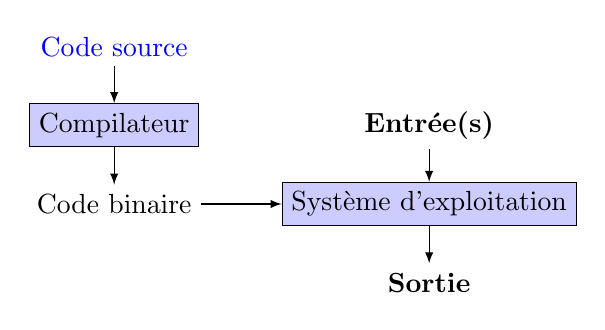
\begin{tikzpicture}
\node (cs) at (0,1) {\textcolor{blue}{Code source}};
\node[draw, fill=blue!20!white] (comp) at (0,0) {Compilateur};
\node (cb) at (0,-1) {Code binaire};
\node[draw, fill=blue!20!white] (se) at (4,-1) {Système d'exploitation};
\node (entree) at (4,0) {\textbf{Entrée(s)}};
\node (sortie) at (4,-2) {\textbf{Sortie}};


\draw[-latex] (cs) -- (comp) ;
\draw[-latex] (comp) -- (cb);
\draw[-latex] (cb) -- (se);
\draw[-latex] (entree) -- (se);
\draw[-latex] (se) -- (sortie);

\end{tikzpicture}  
\caption{Langage compilé}

\end{minipage}\hfill
\begin{minipage}[b]{0.4\textwidth}
\begin{tikzpicture}
\node (cs) at (0,1) {\textcolor{blue}{Code source} };
\node[draw, fill=blue!20!white] (int) at (4,-1) {Interpréteur};
\node (entree) at (4,0) {\textbf{Entrée(s)}};
\node (sortie) at (4,-2) {\textbf{Sortie}};


\draw[-latex,-](cs) -- (0,-1);
\draw[-latex] (0,-1) --(int);
\draw[-latex] (entree) -- (se);
\draw[-latex] (se) -- (sortie);

\end{tikzpicture}  
    \caption{Langage interpreté}
    \label{fig:com}
\end{minipage}
\end{figure}


Avant l'installation, n'oubliez pas de vérifier que Python est bien présent de votre ordinateur.


Une aide à l'installation est disponible sous ce lien :
\url{https://www.commentcoder.com/installer-python/}

Vos professeurs peuvent également vous aider pour installer l'environnement de travail sur votre machine personnelle (très recommandé).

\subsection{Rangement de votre espace de travail}
Tous vos programmes devront être rangés dans des dossiers.
Par exemple, enregistrez votre programme dans un dossier Cours, dans un dossier Semestre 1, dans un dossier Bases de la programmation, dans un dossier tp1.

\subsection{Echauffement}



\subsubsection{Ecrire et lire sur un terminal de commande}


\paragraph{Sortie écran}
Pour afficher une chaîne de caractères en Python 3, ouvrez un éditeur de texte et
écrivez :

\lstinputlisting[language = python]{chapitre1/codes/premier.py}


\begin{enumerate}
    \item Enregistrez ce dossier sous le nom de premier.py
    \item Dans le terminal, exécuter : python3 premier.py
\end{enumerate}

Avec le terminal de commande, allez dans le dossier contenant votre programme.

    \begin{figure}[H]
    \centering
    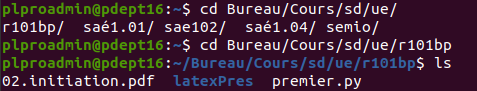
\includegraphics[scale = 0.7]{chapitre1/figures/premier.png}
    \caption{Commandes pour se déplacer dans la hiérarchie de fichiers.}
    \label{fig:enter-label}
\end{figure}

Exécutez le programme avec l'instruction python3 premier.py.

\begin{figure}[H]
    \centering
    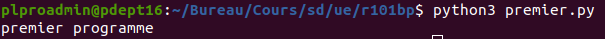
\includegraphics[scale = 0.7]{chapitre1/figures/premier2.png}
    \caption{Commande pour  exécuter un programme.}
\end{figure}



\begin{tcolorbox}[lefttitle=2cm, colframe=gray!75!black, title= \textbf{Exercices}]
A partir du programme premier.py, écrivez les programmes suivant :Exercice


\textbf{1$\diamondsuit$-}
Ecrire le programme  qui ne prend rien en entrée et donne en sortie le texte suivant.
\begin{figure}[H]
    \centering
    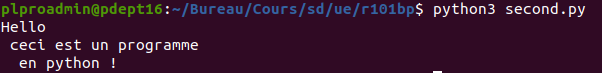
\includegraphics[scale=0.6]{chapitre1/figures/second.png}
\end{figure}
\textbf{2$\diamondsuit$-}
Sauriez-vous le faire en n'utilisant qu'une seule fois l'instruction print ?
\end{tcolorbox}

\paragraph{Entrée utilisateur}


Pour entrer une chaîne de caractères en Python 3, ouvrez un éditeur de texte et
écrivez :

\lstinputlisting[language = python]{chapitre1/codes/programmeAvecEntrees.py}



La sortie écran obtenue est la suivante : 

\begin{figure}[H]
    \centering
    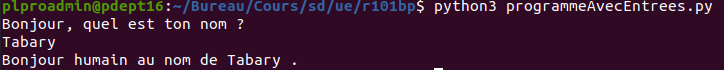
\includegraphics[scale = 0.7]{chapitre1/figures/entree.png}
\end{figure}

\begin{tcolorbox}[lefttitle=2cm, colframe=gray!75!blue, title= \textbf{Tip for Code 1 : "\textit{code is read much more often than it is written}", Guido van Rossum}]


Commentez un paragraphe avec : """.

Commentez une ligne avec : \#.

\textbf{Et quand vous codez, rajoutez des commentaires.}

\url{https://peps.python.org/pep-0008/}

\end{tcolorbox}


\begin{tcolorbox}[lefttitle=2cm, colframe=gray!75!black, title= \textbf{Exercices}]
\textbf{1$\diamondsuit$-}
Ecrire le programme qui donne en sortie le texte suivant.
\begin{figure}[H]
    \centering
    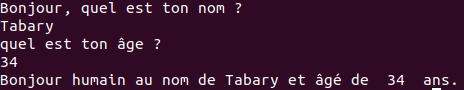
\includegraphics[scale=0.6]{chapitre1/figures/entree2.png}
\end{figure}
\textbf{2$\diamondsuit~\diamondsuit$-}
Modifiez le programme afin d'afficher en plus l'année de naissance.
\begin{figure}[H]
    \centering
    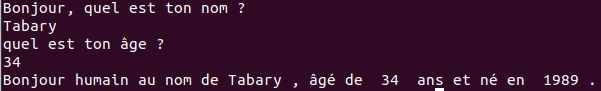
\includegraphics[scale=0.6]{chapitre1/figures/entree3.png}
\end{figure}


\textbf{Aide} : Tip for Code 2 

\textbf{3$\diamondsuit~\diamondsuit~\diamondsuit$ (optionnel)-}
On suppose en plus que la taille est demandée.
L'utilisateur entre un texte qui peut être selon les formats suivants : 177.56cm, ou 177cm, ou 17756cm.
Le terminal répond dans tous les cas :
\begin{figure}[H]
    \centering
    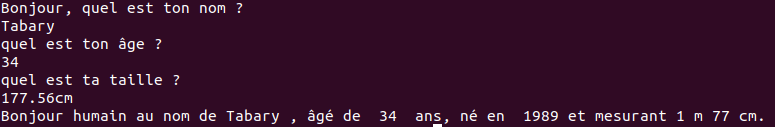
\includegraphics[scale=0.6]{chapitre1/figures/entree4.png}
\end{figure}
\textbf{Aide} : Tip for Code 2 (encore)

\end{tcolorbox}

\begin{tcolorbox}[lefttitle=2cm, colframe=gray!75!blue, title= \textbf{Tip for Code 2 : "\textit{Le shell est votre ami}"}]
Les bugs, ou erreurs de programmation, sont inévitables dans le développement de logiciels complexes, même pour les programmeurs les plus expérimentés.
Il faut savoir lire le code erreur associé.

Une erreur qui risque d'apparaître dans votre cas est la suivante :
\begin{figure}[H]
    \centering
    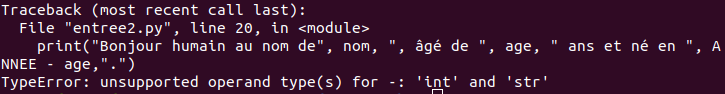
\includegraphics[scale=0.6]{chapitre1/figures/entreeErr.png}
\end{figure}

Dans ce cas, l'erreur se situe \textbf{ligne 20}.

Une variable de type string (texte) est utilisée à la place d'une variable de type int (entier).

En effet ANNEE est une variable globale de type entier (int).
Or, il est impossible de soustraire un texte d'un entier.
Il faut donc changer le type de la variable age afin qu'elle soit un entier.
Cette démarche s'appelle le transtypage.
Pour ce faire, vous pouvez écrire : (int)age.

Source : \url{https://docs.python.org/fr/3/tutorial/inputoutput.html}

\end{tcolorbox}
\subsubsection{Les conditionnelles}
Maintenant, l'objectif est de maîtriser l'alternative\footnote{ \url{https://docs.python.org/fr/3/tutorial/controlflow.html\#if-statements}}.
Testez le programme suivant en respectant bien les indentations.



\lstinputlisting[language = python]{chapitre1/codes/conditionnelle.py}


\begin{tcolorbox}[lefttitle=2cm, colframe=gray!75!blue, title= \textbf{Tip for Code 3 : Indentations et espaces}]

Les annotations pour les variables doivent comporter un seul espace après les deux points.
    Il ne doit pas y avoir d'espace avant les deux points (voir ligne 17).
    Si une affectation a un côté droit, le signe d'égalité doit avoir exactement un espace des deux côtés (voir ligne 11).

Source : Variable Annotations de \url{https://peps.python.org/pep-0008/}

la commande typeof(maVariable) permet de récupérer le type de la variable.

\end{tcolorbox}

\begin{tcolorbox}[lefttitle=2cm, colframe=gray!75!black, title= \textbf{Exercices}]
\textbf{1$\diamondsuit$-}
Ecrire le programme qui spécifie si la personne est mineur, majeure, ou est dans l'année de sa majorité.
\textbf{2$\diamondsuit$-}
Modifier le programme pour incorporer une variale etat qui prend la valeur "mineur", "majeure", ou "est dans l'année de sa majorité", selon l'âge de entrée par l'utilisateur.

\end{tcolorbox}


\subsubsection{Les itératives}
\paragraph{boucle for}
Maintenant, l'objectif est de travailler la boucle for\footnote{ \url{https://docs.python.org/fr/3/reference/compound_stmts.html\#the-while-statement}}.
Testez le programme suivant en respectant bien les indentations.
\lstinputlisting[language = python]{chapitre1/codes/tab.py}

\begin{tcolorbox}[lefttitle=2cm, colframe=gray!75!black, title= \textbf{Exercices}]

\textbf{1$\diamondsuit$-}
Modifier le programme pour incorporer la question pour chaque étudiant "L'étudiant est il venu en cours ? (n/y)".
Si la réponse est "n", alors le prénom de l'étudiant est rajouté à une liste d'étudiants absents.

Ensuite afficher la nouvelle liste des étudiants absents.

\begin{figure}[H]
    \centering
    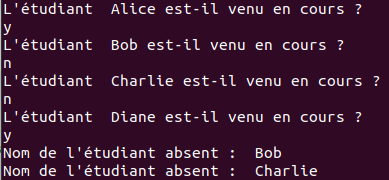
\includegraphics[scale=0.6]{chapitre1/figures/for.png}
\end{figure}
\textit{(optionnel) Quel est, selon la taille de la liste d'entrée, le nombre d'opérations du programme ?}


\textbf{(optionnel) 2$\diamondsuit~\diamondsuit$-}
Réaliser un programme vérifiant qu'aucun étudiant n'est en double dans le tableau.

\textit{ Quel est, selon la taille de la liste d'entrée, le nombre d'opérations du programme ?}

\end{tcolorbox}

\paragraph{Boucle while}
Maintenant, l'objectif est de travailler avec la boucle while\footnote{ \url{https://docs.python.org/fr/3/reference/compound_stmts.html\#the-while-statement}}.

Ce programme modifie le programme précédent afin de s'assurer que l'entrée utilisateur est correcte.
Implémentez-le.
\lstinputlisting[language = python]{chapitre1/codes/while.py}

\begin{tcolorbox}[lefttitle=2cm, colframe=gray!75!black, title= \textbf{Exercices}]

\textbf{1$\diamondsuit$-}
Modifier le programme pour demander si le prénom de l'étudiant présent est bien orthographié.

\textbf{(optionnel)2$\diamondsuit~\diamondsuit~\diamondsuit$-}
Continuer le programme afin de demander une confirmation de l'orthographe avant de valider le prénom.
Modifier le prénom dans la liste s'il était mal orthographié.

\end{tcolorbox}


\subsection{Le juste prix}
Réaliser ce programme :

Un prix caractérisé par une variable globale est déjà présent dans le programme (variable globale). Le but pour l’utilisateur est de deviner ce prix. Chaque fois que l’utilisateur se trompe, l’ordinateur lui dit si c’est plus ou moins que le prix qu’il a donné. Le joueur a gagné une fois qu'il a trouvé le bon prix. Un compteur d'essai donne le nombre de coups nécessaire pour trouver ce juste prix.

\textit{(Optionnel) A votre avis, quelle stratégie de jeu est la meilleure ? et pourquoi sa complexité est de $log (n)$, avec $n$ la taille de la liste ?}


\subsubsection{Réaliser ce programme}

\subsubsection{(Optionnel) Variantes du juste prix}
\paragraph{En entrée, prendre une variable de type entier issue de la librairie random}
\paragraph{En entrée, prendre une voyelle aléatoire (toujours avec la librairie random)}
\paragraph{Avec un nombre de coups limité} Le nombre de coups est défini avec une variable globale.
\paragraph{De faire jouer deux joueurs.} Chacun choisit une lettre de l'alphabet. Le plus rapide à la trouver a gagné.
\paragraph{De faire jouer x joueurs entre eux.} Chacun choisit une lettre de l'alphabet. Le plus rapide à la trouver a gagné. 

\subsubsection{(Optionnel) Générateur des nombres de la suite de Fibonacci}
Sans utiliser de sous-fonction, faite un générateur des nombres de la suite de Fibonacci\footnote{https://fr.wikipedia.org/wiki/Suite\_de\_Fibonacci}.

\newpage

\subsection{Bilan (obligatoire)}



\makebox[0.75\textwidth]{Lors de ce TP, vous vous êtes arrêté à quel exercice ? \enspace\hrulefill}


\makebox[1\textwidth]{Remplir le tableau}

\textbf{Partie savoir faire}
\begin{itemize}
    \item Niveau 1 : Je n'ai pas su l'implémenter. C'est du charabiah pour moi. 
    \item Niveau 2 : J'ai lu le sujet. Les couleurs sont jolies. J'ai fini le premier exercice les yeux rivés sur mon clavier pour chercher les touches. Les erreurs de l'interpréteur me semblent incompréhensibles.
    \item Niveau 3 : J'ai pu avancer à la moitié du sujet, même si c'est difficile et que l'ordi est farceur (comme tous les ordis). Je prends beaucoup de temps à comprendre les erreurs du shell, mais j'y arrive !
    \item Niveau 4 : J'ai complété le TP avec aisance. La plupart des erreurs du shell me sont compréhensibles.
    \item Niveau 5 : J'ai complété le TP, exercices optionnels compris ! J'ai une grande agilité\footnote{agilité $\rightarrow$ ne pas utiliser la souris en codant} quand je code. 
\end{itemize}


\textbf{Partie savoir être}
\begin{itemize}
    \item Niveau 1 :  Pour finir au plus vite, j'élabore des stratégies (copier directement la réponse ou chercher à camoufler le désintérêt : "Si je n'y arrive pas, c'est que le prof n'est pas venu assez vite me donner la solution"). 
    \item Niveau 2 : L'objectif est d'avoir la moyenne sans trop y laisser du temps ou de l'énergie. Je suis bien obligé de faire le TP, même si l'idée de me servir du pannel de ressources me semble saugrenue. Si c'est possible de récupérer la réponse (ou de suivre à côté d'un camarade\footnote{Mais si, c'est du travail d'équipe : il code et je le soutiens émotionnellement !}), alors je ne dirai pas non. 
    \item Niveau 3 : Je prends doucement mes marques. Je me suis servi de façon hésitante de plusieurs ressoures dispos (shell, camarades, enseignants, manuel, sites web, ou même canard\footnote{\url{https://fr.wikipedia.org/wiki/M\%C3\%A9thode_du_canard_en_plastique}}) en cherchant à comprendre leur réponse. J'aimerais un jour pouvoir développer  mes propres projets et il faut pour cela que je gagne en autonomie.
    \item Niveau 4 :   Je suis autonome dans l'utilisation des ressoures disponibles (shell, camarades, enseignants, manuel, sites web, ou même canard\footnotemark[7]). J'ai même un projet personnel en cours que j'aimerais finir.
    \item Niveau 5 : J'évolue avec aisance dans cet environnement ! Je  fais même partie dorénavant des ressoures dispos et  j'échange facilement sur ces notions. J'ai plusieurs projets informatiques personnels. 
\end{itemize}

\begin{table}[H]
    \centering
    \begin{tabular}{|c|c|c|} \hline
        \textbf{Notions} & \textbf{Niveau atteint} (de 1 à 5) \textbf{Savoir faire}  & \textbf{Niveau atteint} (de 1 à 5) \textbf{Savoir être}\\\hline
        Instructions simples & & \\\hline
        Variables &&\\\hline
        Conditionnelles &&\\\hline
        Boucle For &&\\\hline
        Boucle While && \\\hline
        Respect des règles de bon codage && \\\hline
    \end{tabular}
\end{table}



\begin{tcolorbox}[lefttitle=2cm, colframe=gray!75!green, title= \textbf{SUPER TIP}]

Pour finir, un site pour s'entraîner/tester les instructions. En français.

Source : \url{https://www.geeksforgeeks.org/python-tuples/?ref=lbp}
\end{tcolorbox}

